\let\negmedspace\undefined
\let\negthickspace\undefined
\documentclass[journal]{IEEEtran}
\usepackage[a5paper, margin=10mm, onecolumn]{geometry}
\usepackage{tfrupee} 

\setlength{\headheight}{1cm} 
\setlength{\headsep}{0mm}     

\usepackage{gvv-book}
\usepackage{gvv}
\usepackage{cite}
\usepackage{amsmath,amssymb,amsfonts,amsthm}
\usepackage{algorithmic}
\usepackage{graphicx}
\usepackage{textcomp}
\usepackage{xcolor}
\usepackage{txfonts}
\usepackage{listings}
\usepackage{enumitem}
\usepackage{mathtools}
\usepackage{gensymb}
\usepackage{comment}
\usepackage[breaklinks=true]{hyperref}
\usepackage{tkz-euclide} 
\usepackage{listings}                                        
\def\inputGnumericTable{}                                 
\usepackage[latin1]{inputenc}                                
\usepackage{color}                                            
\usepackage{array}                                            
\usepackage{longtable}                                       
\usepackage{calc}                                             
\usepackage{multirow}                                         
\usepackage{hhline}                                           
\usepackage{ifthen}                                           
\usepackage{lscape}

\begin{document}

\bibliographystyle{IEEEtran}
\vspace{3cm}

\title{1.6.23}
\author{AI25BTECH11008 - Chiruvella Harshith Sharan}
{\let\newpage\relax\maketitle}

\renewcommand{\thefigure}{\theenumi}
\renewcommand{\thetable}{\theenumi}
\setlength{\intextsep}{10pt} 

\numberwithin{equation}{enumi}
\numberwithin{figure}{enumi}
\renewcommand{\thetable}{\theenumi}

\textbf{Question}: Are A(3,1), B(6,4) and C(8,6) collinear?\\\\

\textbf{Solution:}\\

We check collinearity using vector method.  

\[
\vec{B}-\vec{A} = \myvec{6-3 \\ 4-1} = \myvec{3 \\ 3}
\]  

\[
\vec{C}-\vec{A} = \myvec{8-3 \\ 6-1} = \myvec{5 \\ 5}
\]  

Now form the matrix:  

\[
\vec{M} = \myvec{\vec{B}-\vec{A} & \vec{C}-\vec{A}}^T 
= \myvec{3 & 5 \\ 3 & 5}
\]  

Clearly, both rows are multiples of each other, so  

\[
\text{rank}(M) = 1
\]  

\[
\therefore \; A(3,1), \, B(6,4), \, C(8,6) \; \text{are collinear.}
\]

\begin{figure}[htbp]
    \centering
    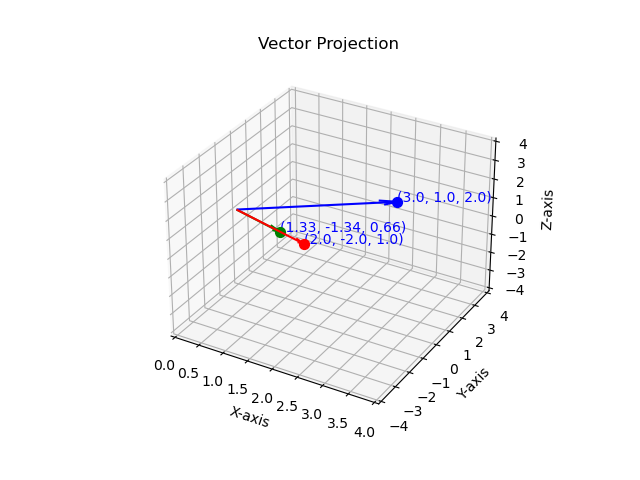
\includegraphics[width=0.8\linewidth]{figs/fig1.png}
    \caption{Graph showing collinear points A, B, C}
    \label{fig:fig/fig1.png}
\end{figure}

\end{document}
